\chapter{3D hand pose reconstruction}

\section{Overview of proposed methods}

The work is aimed at solving three tasks: studying the influence of preliminary frames on the reconstruction of video sequences; investigating the process of results refinement; image reconstruction of hands displaying the letters of American Sign Language. We are solving all by the introduced 3-stage computational pipeline, where every stage is a neural network designed to solve a small task.

The proposed method can be described by the schema of 3D hand pose estimation close to specified in Fig 2.4. Except it does not have the first stage of the hand localization stage and work directly with centered hands. In that way, the introduced method can be generalized to the sequence of architectures A, B, and C. We sequentially compute locations of 2D key-points by network A, depth for each key point by B, and after that, calculate the vector of MANO parameters from key points by C. 

In total, 13 ANN architectures were tested for tasks A, B, and C combined. Six designs were studied as candidates for network A, five - for B, and two for C. The networks A and B can be considered as one architecture for 3D key-point detection. For A and B, we were focused on the influence of two factors on the training process. Those factors are additional frames at input and refinement of predictions. To investigate the difference in the training trends was developed a system for parallel training and evaluation of multiple networks. Network C stands alone from networks A and B because it doesn't process images. Its task is to estimate the vector of MANO hand surface generation parameters from a set of 3D points. This stage finishes the computational pipeline, which allows us to annotate a subset of American Sign Language.

\section{Neural networks for 2D key point detection}

Network A takes as an input RGB information and outputs 22 heatmaps of size 224x224, \{H1, H2,..., H2\}, where each heatmap Hk from indicates the probability of observing the kth keypoint and for k=22 probability of no key points. A similar approach has proven to work efficiently in \cite{PCP}.

\begin{figure}
\caption{Building blocks and assembled networks for 2D key point detection: a)U-Net architecture; b)Hourglass Like Module c)Architecture of STH\_2; d)Architecture of STH\_3.}
\centering
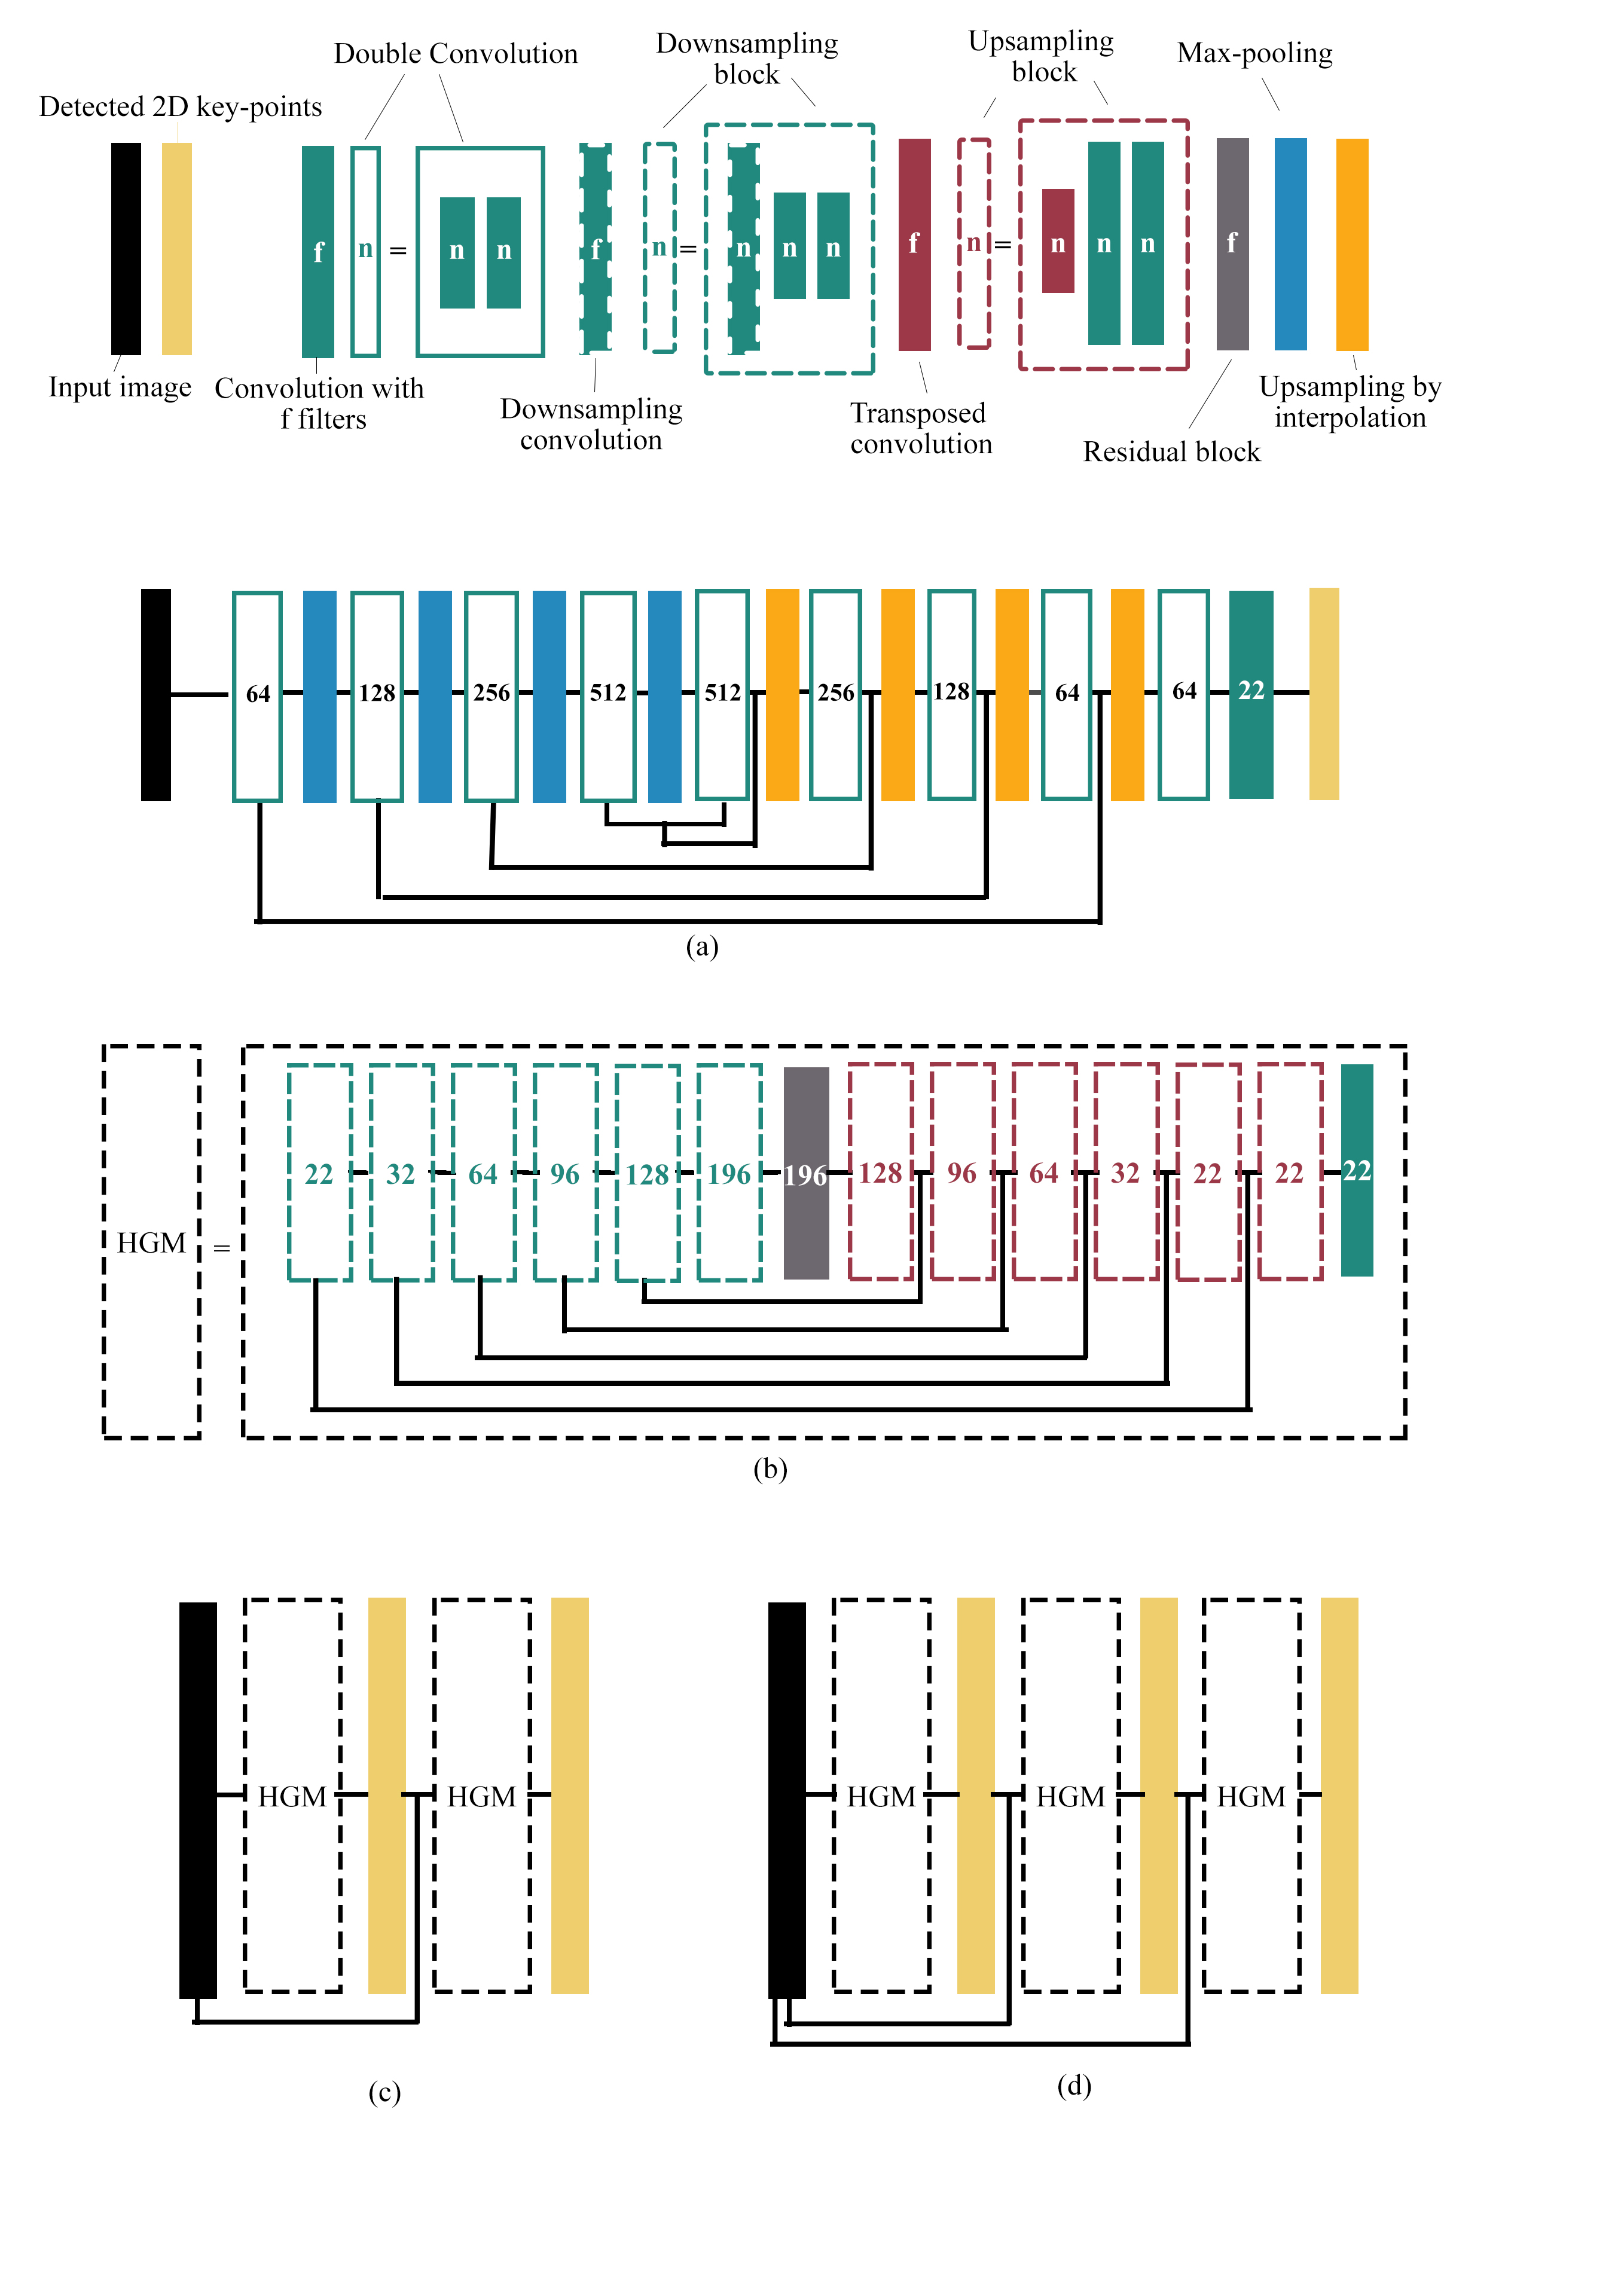
\includegraphics[width=1\textwidth]{finala}
\end{figure}

Two Stacked Hourglass Like and one U-Net architecture are candidates for main network at stage A for 2D key-point detection. Each candidate has a variation for video and image processing. In total, there are 6 architectures for 2D key point localizations with the following id’s: UNET\_VID, STH\_2\_VID, STH\_3\_VID, UNET\_PIC, STH\_2\_PIC, STH\_3\_PIC. Where ‘STH\_’ stands for Stacked Hourglass like architecture; \_VID means that input contains concatenated RGB frames and 2D points of the previous frame;  \_PIC means that input contains a single RGB image.

Let kc denote the convolutional layer with k filters and stride 1, kd - the convolutional layer with k filters and stride 2, ku - the transposed convolutional layer with k filters and stride 2, kfc - fully connected layer with k neurons, mp - max pooling with 2x2 filter, up2 is x2 upsampling by interpolation, kr - residual block from Fig 2.2 with k filters. All convolutional layers except for the last one are followed by batch normalization and ReLU activation.

Implementation of U-Net is: 64c, 64c, mp, 128c, 128c, mp, 256c, 256c, mp, 512c, 512c, mp, 512c, 512c, up2, 256c, 256c, up2, 128c, 128c , up2, 128c, 128c, up2, 64c, 64c, up2, 64c, 64c, 22c. Outputs of layers are concatenated in order shown in Fig. 3.1 a).

The architecture of proposed HGM is: 22d, 22c, 22c, 32d, 32c, 32c, 64d, 64c, 64c, 128d, 128c, 128c, 196d, 196c, 196c, 196r, 128u, 128c, 128c, 96u, 96c, 96c, 64u, 64c, 64c, 32u, 32c, 32c, 22u, 22c, 22c, 22u, 22c, 22c, 22c. Outputs of layers summed in order shown in Fig. 3.1 b). 

The architecture of STH\_2 consist of two hourglass modules where the second module takes as input image concatenated with the initial prediction from the first module, as illustrated in Fig 3.1 c). The architecture of STH\_3 set in the same way as STH\_2, except there is one additional module for refinement, as shown in Fig 3.1 d).

It is important to accentuate that architectures drastically differ in size. 

\begin{table}[H]
\small
\begin{tabularx}{1\textwidth}{sbbb}
 \hline
 net\_id & num\_of\_parameters & num\_of\_refinements & skip-connection type \\
 \hline
STH\_2\_PIC &
6106056 &
2 &
addition
\\
\hline
STH\_2\_VID &
6115956 &
2 &
addition 
\\
\hline
STH\_3\_PIC &
9161262 &
3 &
addition 
\\
\hline
STH\_3\_VID &
9176112 &
3 &
addition 
\\
\hline
UNET\_PIC &
13396694 &
1 &
concatenation
\\
\hline
UNET\_VID &
13411094  &
1 &
concatenation
\\
\hline
\end{tabularx}
\caption{\label{tab:res_0}Differences between nets A}
\end{table}


\section{ANN for depth estimation (Network B)}

Network B is used for the estimation of 21 depth values for each key point. We propose 5 architectures for depth estimation marked as B\_PIC, B\_VID, B\_R\_PIC, B\_R\_VID, AB\_PIC. Where B\_R means that output is calculated multiple times (refined), AB stand for additional usage of features from network A, \_VID means that input contains concatenated RGB frames and 2D points from current and previous frame, as well as depth from the previous frame;  \_PIC means that input contains concatenated RGB data with 2D key points from a single image. 

\begin{figure}
\caption{Studied building blocks and networks for depth estimation: a)Feature Extractor; b)Dense layers with additional depth inputs; c)Dense layers with additional depth outputs.}
\centering
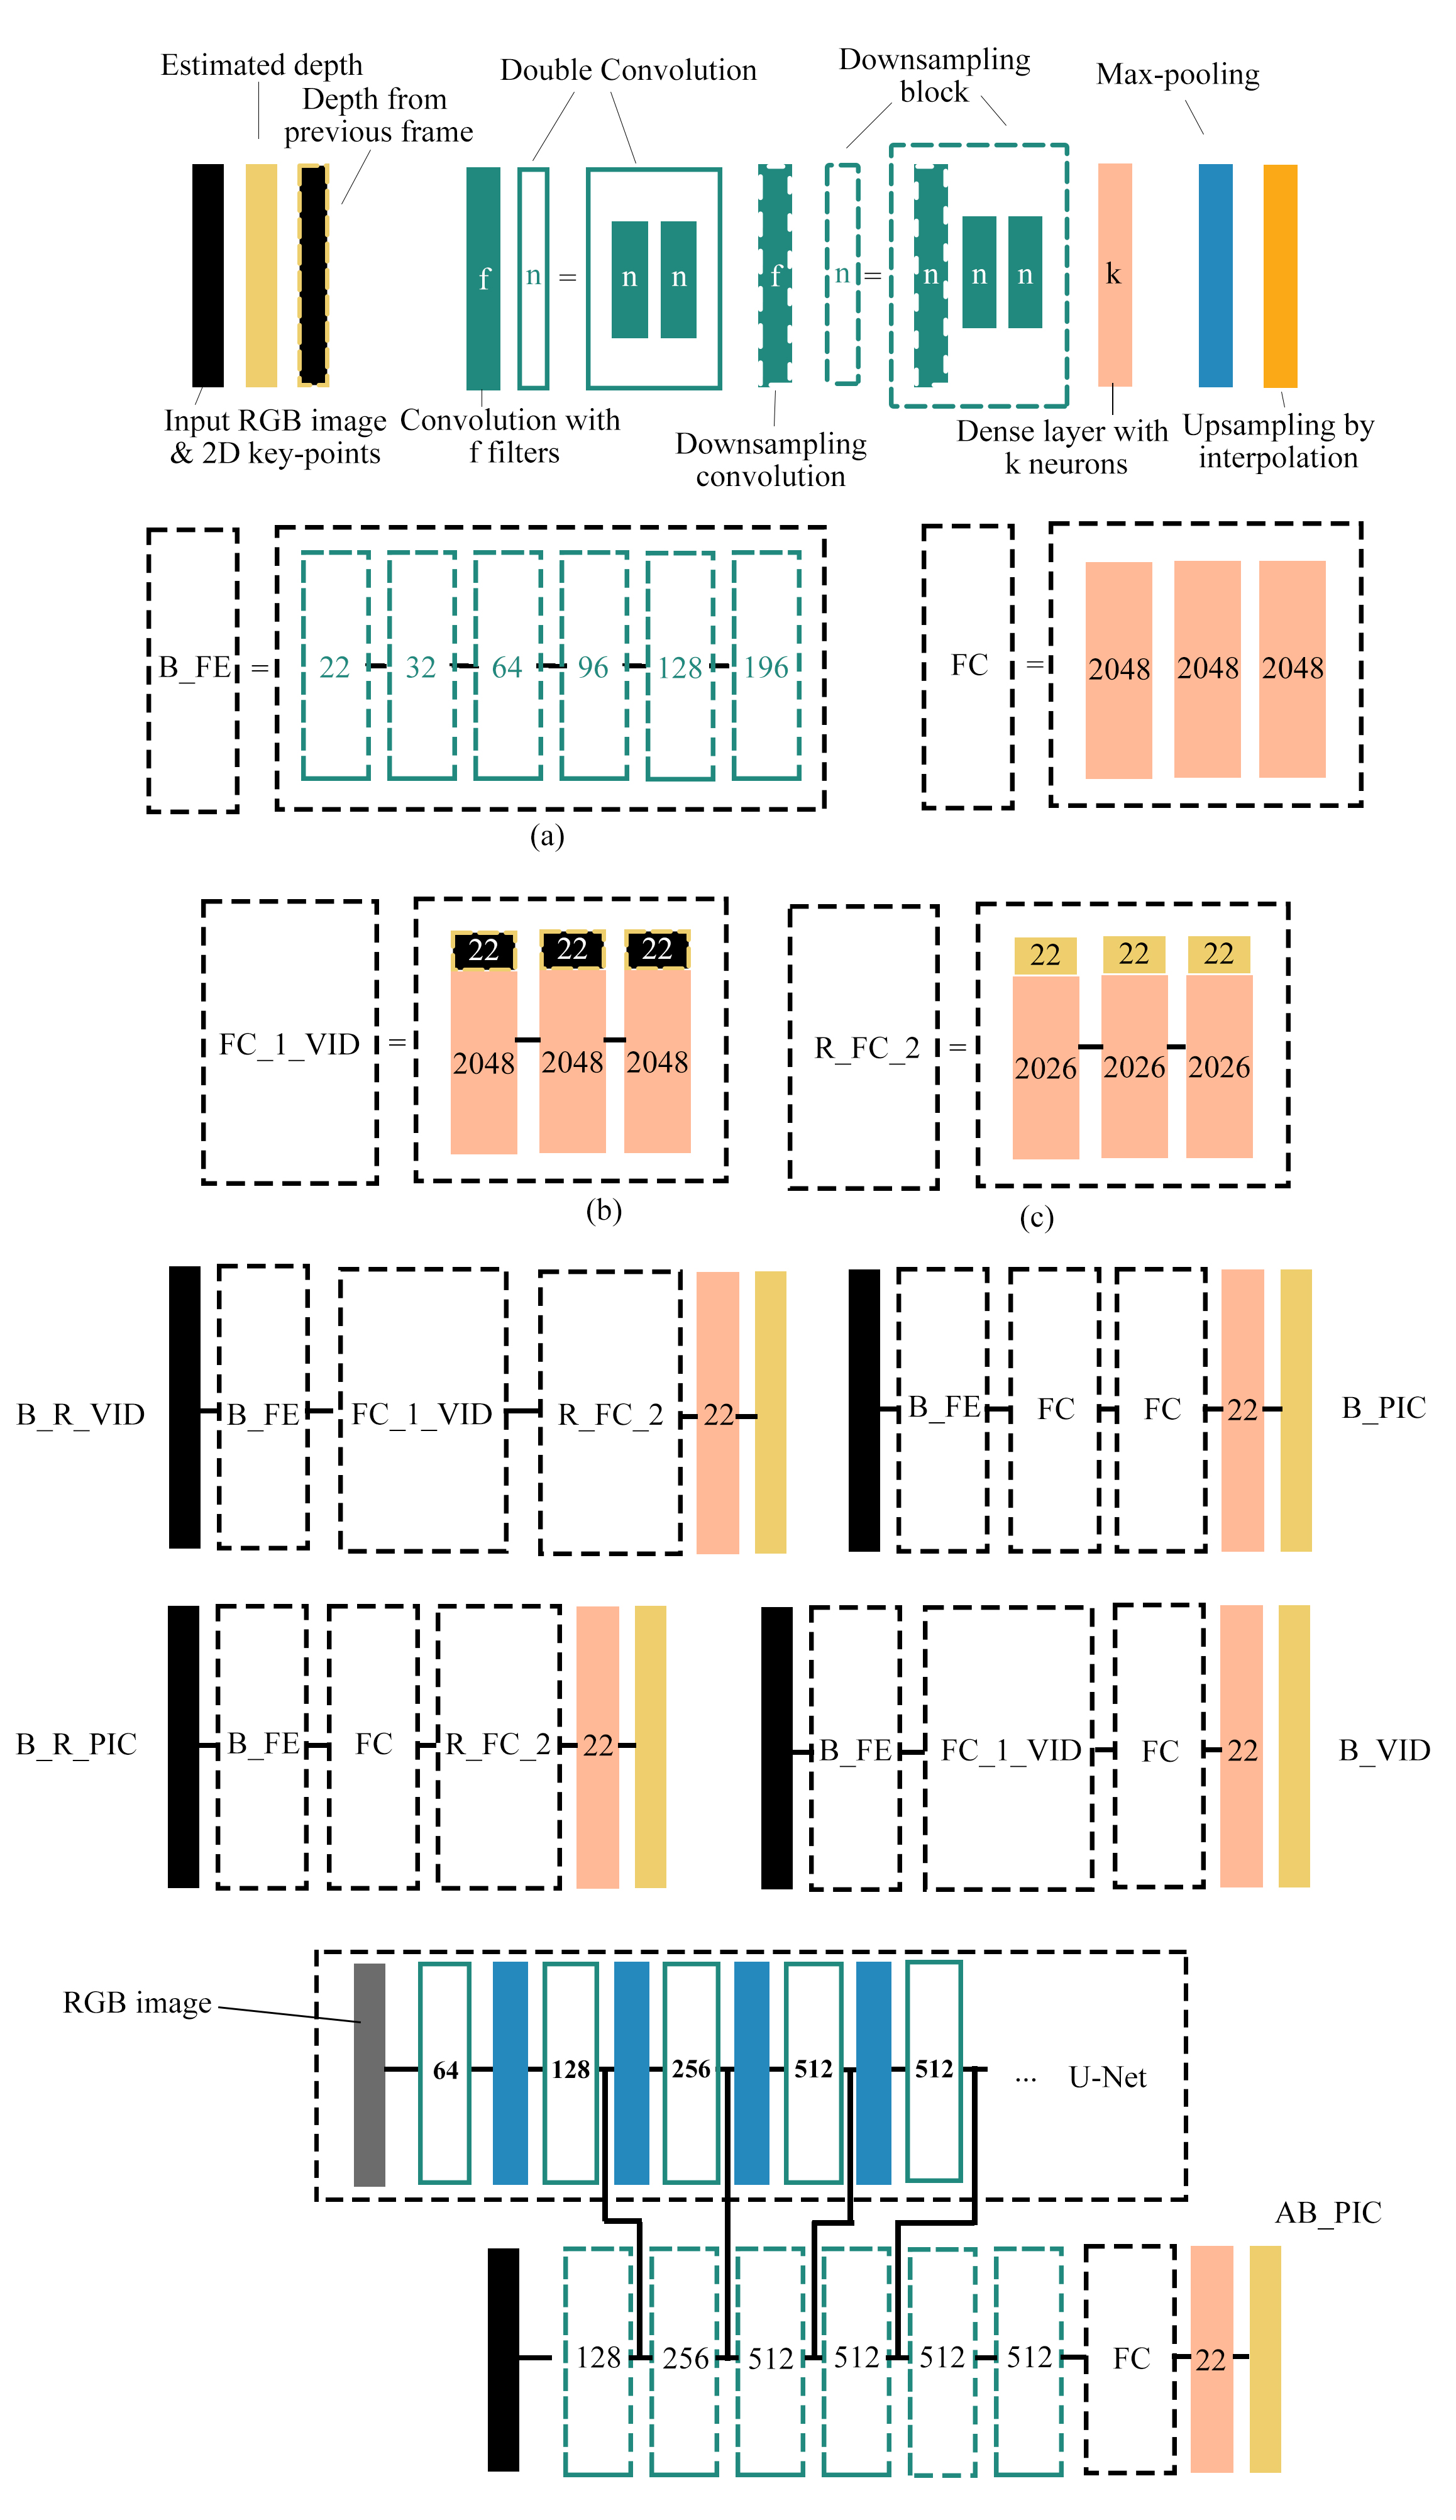
\includegraphics[width=1\textwidth]{finalb}
\end{figure}

All networks have two parts. The first part is Feature Extractor (FE), and the second is a set of fully connected blocks (FC). The set of convolutional layers followed by dense layers is an effective solution for the image to vector problems \cite{m2}. Architecture of FE is same for B\_PIC, B\_VID, B\_R\_PIC, B\_R\_VID: 16d, 16c, 16c, 32d, 32c, 32c, 64d, 64c, 64c, 128d, 128c, 128c. Feature Extractor of network with id AB\_PIC has following architecture: 128d, 128c, 128c, 256d, 256c, 256c, 512d, 512c, 512c, 512d, 512c, 512c, 512d, 512c, 512c, 512d, 512c, 512c. Outputs of Feature Extractor layers for network AB\_PIC concatenated with outputs of UNET layers in a way shown at Fig. 3.2
    

Sets of fully connected blocks are different for all networks. Networks B\_PIC, B\_VID, B\_R\_PIC, B\_R\_VID ends with 7 dense layers. Networks that work with video sequences have additional inputs at first three blocks, as shown at pic 3 b). Id's of networks with refinement of results marked with \_R and optimized so that each of 4 ending layers has 22 neurons responsible for depth info. Network AB\_PIC has 4 fully connected layers with no additional info or refinement, and the output of the last layer only is depth.

\section{Network for estimation of shape parameters}

The 3D shape of a hand is represented as a mesh with 778 vertices. Those vertices are encoded in 51 parameters and decoded by the MANO model. We convert 21 3D key-points into MANO parameters by network C.
    
\begin{figure}[h]
\caption{Studied architectures for shape parameterization. a) Shema of MANO input-output mapping; b)Architecture of C\_RNN network; c)Architecture of C\_MLP network.}
\centering
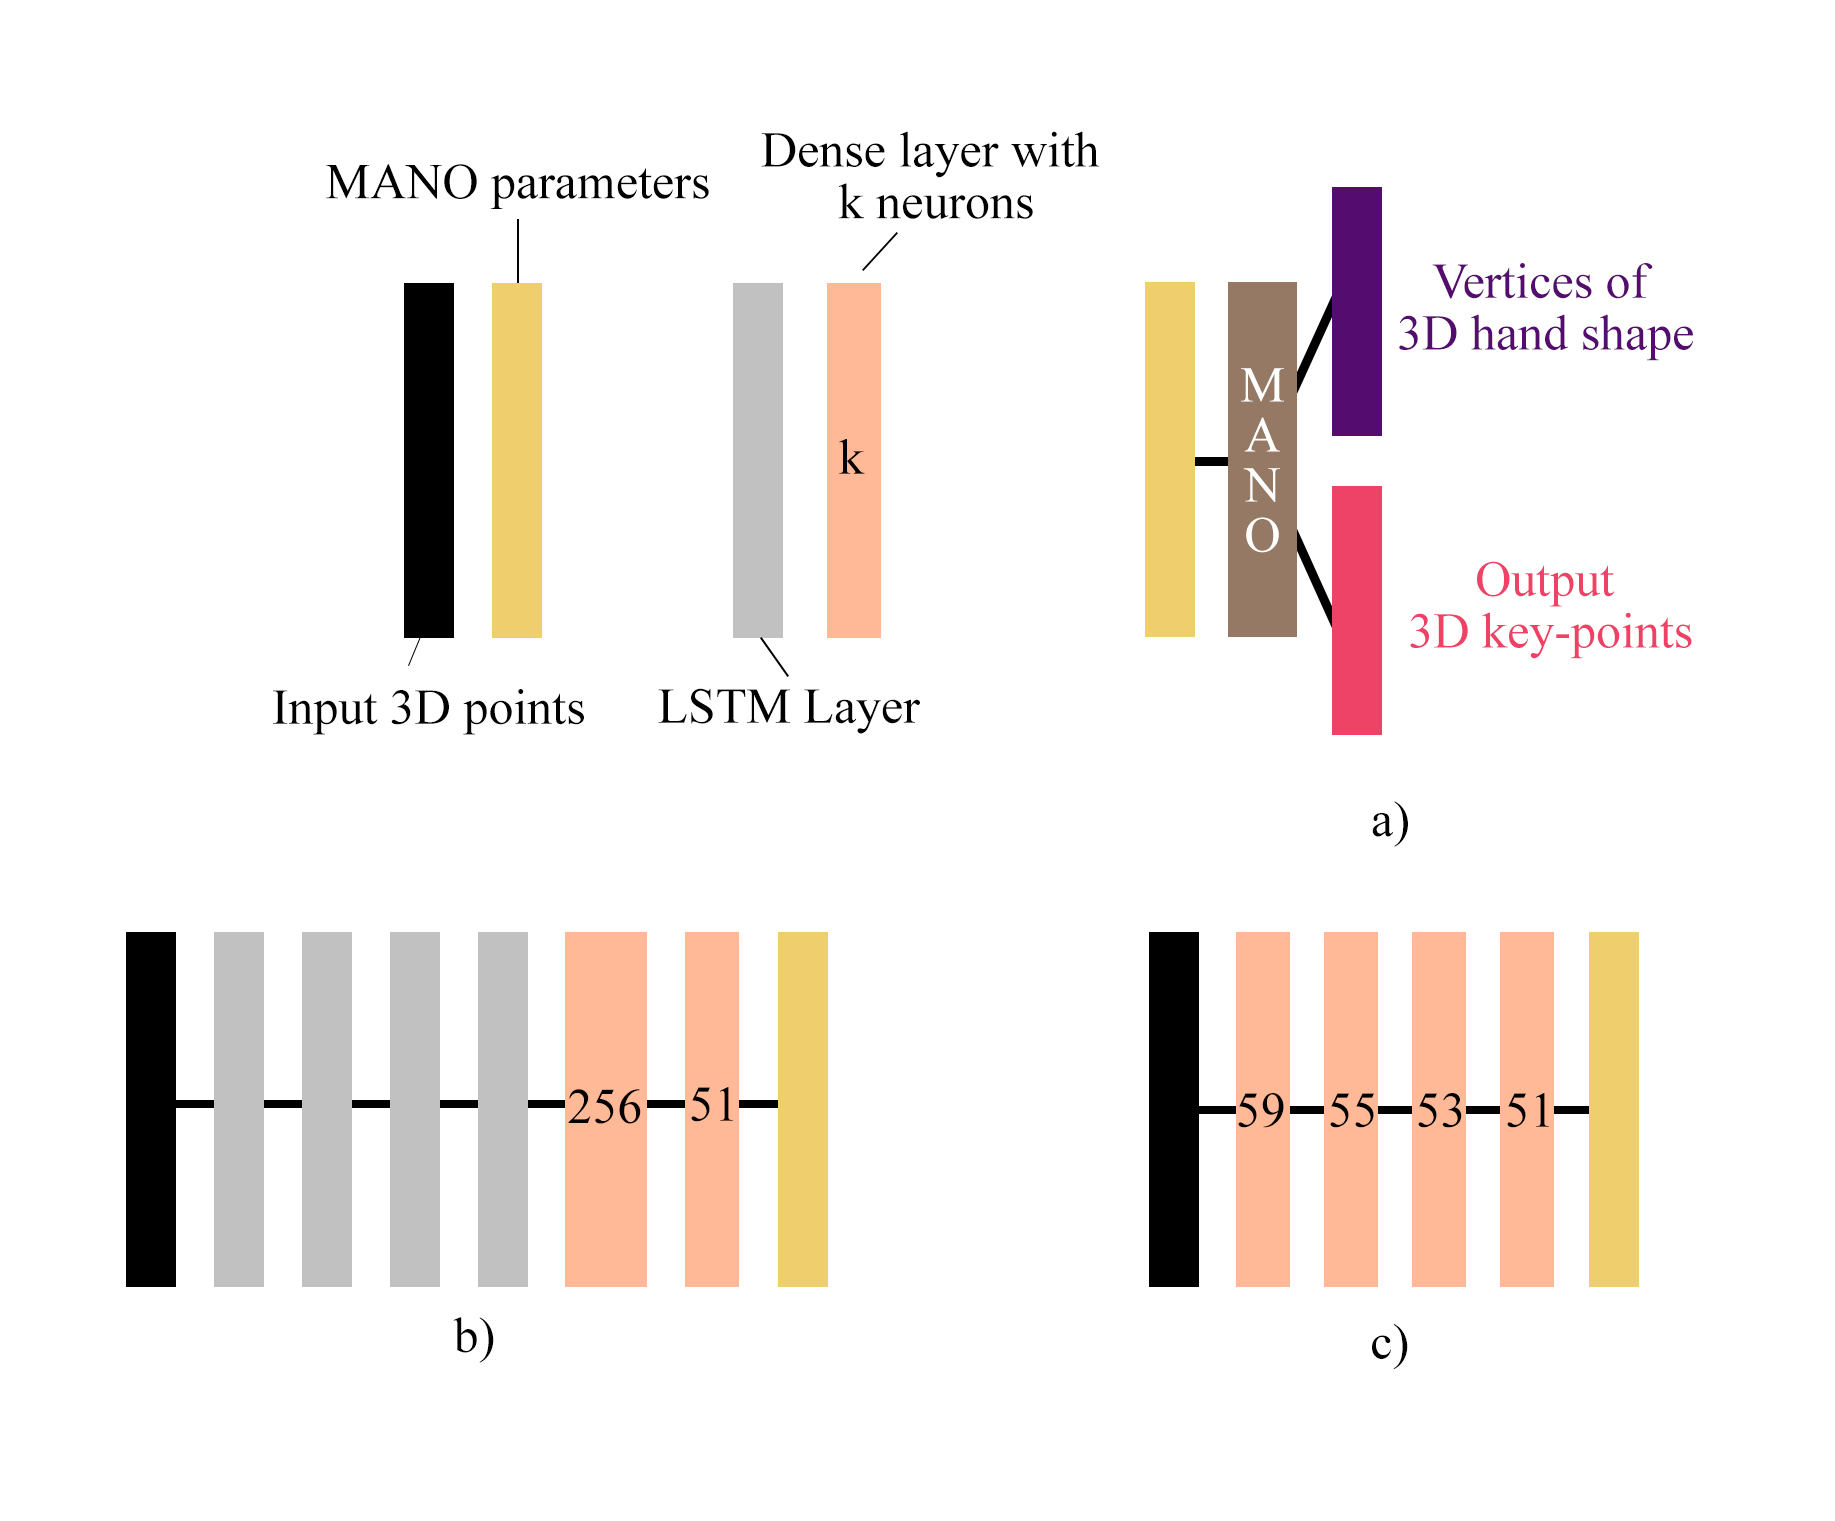
\includegraphics[width=0.6\textwidth]{finalc}
\end{figure}


We considered two architectures as candidates for network C. The first model has id 'C\_RNN' and consists of 4 LSTM layers and fully connected output. The second model with id 'C\_MLP' is a set of fully connected layers. Illustrated in Fig. 3.3.
 



